\documentclass[a4paper,8pt,hyperref, twocolumn, aps, prl]{article}

\title{\bfseries \Large 
%Surface second harmonic generated by submilliwatt pump
%Surface second-order nonlinear effects with ultralow power
%Ultralow-pumped surface second-harmonic generation in centrosymmetric medium
Surface second-harmonic generation enhanced by an ultrahigh-$Q$ microresonator
%of nonpolar media
}
\author{\normalsize  Xueyue Zhang$^{1,2}$, Qi-Tao Cao$^{1}$, Yu-xi Liu$^{2,3}$, Qihuang Gong$^{1,4}$, Yun-Feng Xiao$^{1,4,*}$ \\
  \\
\normalsize $^1$ State Key Laboratory for Mesoscopic Physics and School of Physics, Peking University \\
\normalsize Collaborative Innovation Center of Quantum Matter, Beijing 100871, People's Republic of China \\
\normalsize $^2$ Department of microelectronics and nanoelectronics, Tsinghua University, Beijing 100084, People’s Republic of China \\
\normalsize $^3$ Institute of Microelectronics, Tsinghua University, Beijing 100084, People’s Republic of China \\
\normalsize $^4$ Collaborative Innovation Center of Extreme Optics, Taiyuan 030006, Shanxi, People’s Republic of China \\
\normalsize $^*$ E-mail: yfxiao@pku.edu.cn
}
\date{\normalsize \today}

\usepackage[left=16mm,right=16mm, bottom = 16mm, top=20mm]{geometry}
\usepackage{upgreek}
\usepackage{hyperref}
\usepackage{booktabs}
\usepackage{tabularx}
\usepackage{xtab}
\usepackage{graphicx}
\usepackage{listings}
\usepackage{url}
\usepackage{amsmath}
%\usepackage{nature}



\lstset{
	flexiblecolumns,
	basicstyle = \sffamily,
	keywordstyle = \bfseries,
	commentstyle = \rmfamily\itshape,
	stringstyle = \ttfamily
}

\hypersetup{colorlinks=false}



%\pagestyle{myheadings}
%\markright{Name: Xueyue Zhang, GTID: 903181650}

\bibliographystyle{naturemag}

\begin{document}

\maketitle


\textbf{
Second-order nonlinear optical processes lie in the heart of many applications in both classical and quantum regime, e.g. frequency conversion,  quantum squeezing and entanglement \cite{boyd2003nonlinear, pereira1988generation, kwiat1995new}. 
Inversion symmetry inhibits the second-order nonlinear dipole response in plenty of materials widely used in integrated photonics such as SiO$_2$, Si and Si$_3$N$_4$ \cite{boyd2003nonlinear, leuthold2010nonlinear, moss2013new}.
Symmetry breaking at surfaces/interfaces can produce second-order nonlinearity \cite{shen1989surface, heinz1991second, bloembergen1968optical, cazzanelli2016second}, but its signal requires high-power excitation and is hard to be distinguished from the contribution of bulk multipole nonlinearity \cite{heinz1991second, sun2015surface}. 
Here, for the first time, we report second harmonic generation (SHG) originating deterministically from the surface nonlinearity of a silica microcavity.
The bulk multipole nonlinear effects are eliminated via pumping a fundamental mode with transverse electric polarization, enabling the identification of surface nonlinear response.
The doubly resonant enhancement of ultrahigh-$Q$ cavity modes lowers the pump power below one milliwatt, and boosts the SHG conversion efficiency to $0.049\%$ W$^{-1}$, around $14$ orders of magnitude larger compared with the non-resonance case \cite{tian2014recent}. 
This work can trigger intense applications in ultra-sensitive surface analysis, extend the frequency conversion range of silica photonic devices and possibly push the surface nonlinear effects into the quantum regime.
}

The second-order nonlinearity in materials with inversion symmetry originates from both the asymmetric potential experienced by the surface/interface layer and the bulk multipole response beyond the electric-dipole approximation \cite{shen1989surface, heinz1991second}. 
Different from breaking the bulk inversion symmetry, e.g. exerting external strain \cite{jacobsen2006strained, cazzanelli2012second} or electric field \cite{timurdogan2017electric}, the second harmonic and sum frequency generation induced by the intrinsic surface nonlinearity have been developed as a non-invasive label-free probe, for example, in detecting the arrangement,  adsorption or reaction of molecules on the surface \cite{sun2015surface, heinz1983determination, corn1994optical}.  
%For , second harmonic and sum-frequency generation spectroscopy has been developed into a viable surface analytical tool 
However, the signals from surface nonlinear effects are extremely weak even under the high-intensity pump, typically only thousands of second-harmonic photons generated from a $50$-fs pulse with $500$ GW/cm$^{2}$ \cite{tian2014recent}. 
Additionally, the bulk multipole second-order effects disturb the deterministic study of surface properties, which has long been highly challenging \cite{heinz1991second, tian2014recent}.

In the past decades, cavity-enhanced nonlinear optics with low pump power has witnessed dramatic development in whispering-gallery (WG) microresonators, with the demonstration of Raman laser \cite{spillane2002ultralow}, harmonic emission \cite{ilchenko2004nonlinear, carmon2007visible, furst2010naturally} and optical frequency combs \cite{del2007optical}. 
The second-order nonlinear signal was also observed
in cavities made of centrosymmetric materials \cite{gouveia2013second, lettieri2002second, lettieri2005second, levy2011harmonic, asano2016visible, xue2017second}.
These studies, however, fail to clarify the surface second-order nonlinear effect and to operate under low pump power, which present obstacles in surface physics and further applications.
Here, we observe second harmonic, originating from surface-induced symmetry breaking and bulk multipole response (Fig. \ref{pic:Fig1}a), in a silica WG microsphere under the continuous wave pump below 1 mW. 
A conversion efficiency of $0.049\%$ W$^{-1}$ benefits from doubly resonant enhancement of ultrahigh-$Q$ modes (also known as perfect phase match), which is achieved by thermal effect and optical Kerr effect. 
We further confirm the second-order nonlinear signal only from the symmetry breaking at the surface, by analyzing the polarization dependence and the electric field distribution of the pump mode. 

\begin{figure*}[!ht]
\centering
%\captionsetup{singlelinecheck=no, justification = RaggedRight}
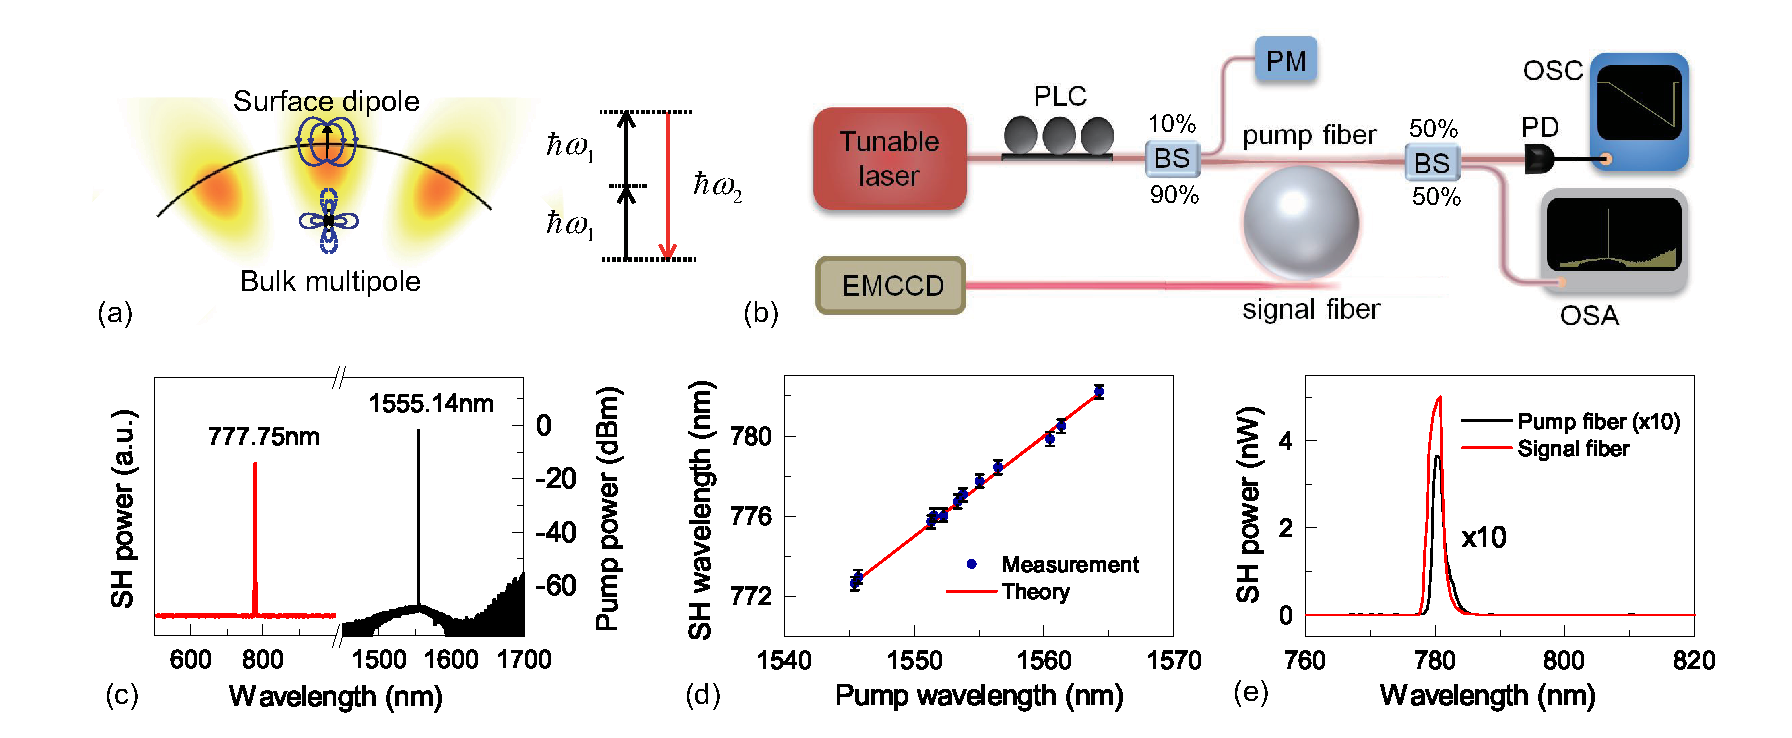
\includegraphics[width=18cm]{Fig1.eps}
\caption{\textbf{Experimental set-up and observation of cavity-enhanced SH signals. a, }SH is generated from the surface dipole response and the bulk multipole response in a WG microsphere. \textbf{b, }The pump light from a tunable laser around 1550 nm is coupled into a silica microsphere through a tapered fibre, and a second fibre is used to collect the SH signal. OSC: oscilloscope. OSA: optical spectrum analyzer. PLC: polarization controller. BS: beam splitter. EMCCD: electron-multiplying CCD. \textbf{c, }Measured SH spectrum (red) and the corresponding pump spectrum (black). \textbf{d, }Measured SH wavelengths versus the corresponding pump wavelengths when different modes are pumped. \textbf{e, }Comparison of SH power collected by signal fibre and pump fibre (10 times magnified).}
\label{pic:Fig1}
\end{figure*}


In the experiment, a silica microsphere (diameter $\sim$ $62$ $\upmu$m) 
is pumped through a tapered optical fibre (waist diameter $\sim$ $1$ $\upmu$m) at $1550$ nm band, as shown in Fig. \ref{pic:Fig1}b. To collect SH signal efficiently, a second fibre taper (waist diameter $\sim$ 0.5 $\upmu$m) designed for 780 nm band is incorporated into the system. The intrinsic quality factor for the pumped cavity mode is $4.8\times10^7$. 
Figure \ref{pic:Fig1}\textbf{c} shows a typical SH spectrum measured from the electron-multiplying CCD (EMCCD) and the corresponding pump spectrum from the optical spectrum analyzer (OSA). The SH signal appears at $777.75$ nm when pumped at $1555.14$ nm, which deviates only $0.023$\% from the expected wavelength, falling into the resolution tolerance of OSA and EMCCD spectrometer.
Note that stimulated Raman scattering and parametric oscillation do not occur because their thresholds are far above the pump power in the experiment \cite{spillane2002ultralow, del2007optical}. 
Third harmonic generation is also absent due to the phase mismatch in the nonlinear optical process \cite{carmon2007visible}.
Moreover, SH signals arise frequently when cavity modes are pumped from $1545$ nm to $1565$ nm, as shown in Fig. \ref{pic:Fig1}d.
Among the occurrence of SH, a maximum signal power of $5$ nW is observed via the signal fibre. To compare the collecting efficiency of the two fibres, we optimize the fibre-cavity coupling so that the SH signal from the pump fibre is also observable, but the maximum signal power is still over one order of magnitude weaker than that from the signal fibre. From either fibres, SH signal is absent when the pump is off-resonance with cavity modes, which helps to eliminate the possibility of spurious signals such as the second-order diffraction of the EMCCD grating.


The doubly resonant enhancement plays a pivotal role in efficient SHG, which is achieved by perfect phase-matching including momentum conservation and energy conservation \cite{boyd2003nonlinear}.
The former can be fulfilled by a pair of modes with proper angular momentum relation $m_2=2m_1$, where $m_1$ ($m_2$) is the azimuthal number of the pump (SH) cavity mode. 
The material and geometric dispersion presents a challenge on energy conservation, obstructing the double resonance $\omega_2=2\omega_1$ and consequently, efficient SHG. 
More accurately, the SH power can be derived from coupled mode equations (see Supplementary Information)
\begin{equation}
P_2 = \frac{4|g|^2\kappa_{2e}Q_2^2/\omega_2^2}{4Q_2^2(2\omega_p/\omega_2-1)^2+1}\frac{16\kappa_{1e}^2Q_1^4/\omega_2^4}{[4Q_1^2(\omega_p/\omega_1-1)^2+1]^2}P_1^2,
\label{eq:P2P1}
\end{equation}
where the subscripts $j=1, 2$  represent the pump cavity mode and SH mode respectively with $\omega_j$ being the resonant frequency and $Q_j$ the loaded quality factor, $\omega_p$ and $P_1$ denotes the pump frequency and power respectively, $g$ is the second-order nonlinear coupling strength between the two modes, and $\kappa_{je}$ represents the external coupling rate. The pump power depletion is ignored due to the weak second-order nonlinear effect in silica.
Equation (\ref{eq:P2P1}) shows that ultrahigh $Q$ is indispensable in boosting the SH power, while it also presents a challenge to achieve the double resonance due to the aggravated influence from frequency mismatch. 
In order to compensate the dispersion, delicate geometric control and the integration of fine nanostructures were proposed in the cavities \cite{levy2011harmonic, kozyreff2008whispering, xu2008second, dominguez2011whispering}, but challenging for an ultrahigh-$Q$ (ultra-narrow-linewidth) microresonator.  
To tune the cavity dispersion precisely and dynamically, we leverage the cavity-enhanced thermal and optical Kerr effects to manipulate the frequencies of both pump and SH cavity modes. 


\begin{figure*}[!ht]
\centering
%\captionsetup{singlelinecheck=no, justification = RaggedRight}
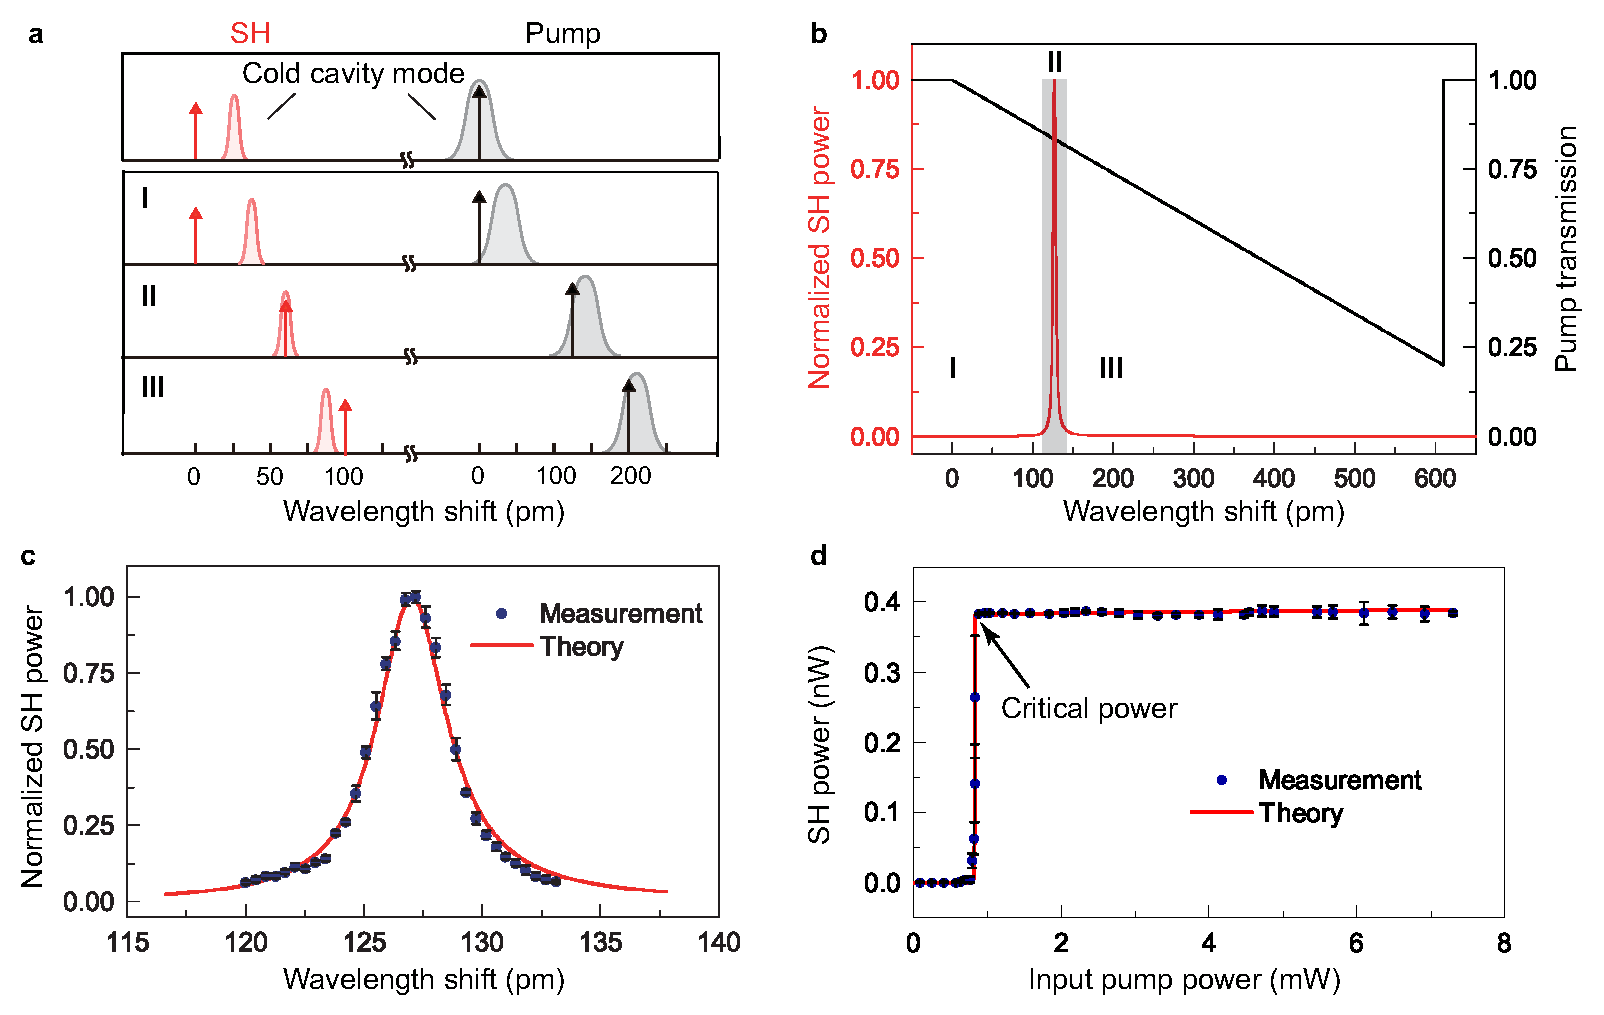
\includegraphics[width=17cm]{try_ed3.eps}
\caption{\textbf{Thermal effect and Kerr effect assisted phase-matching. a, }Schematic of the phase-matching process. Detuning here is the wavelength relative to the cold-cavity wavelength of the pump mode (to half of this wavelength for SH detuning). The black (red) arrow represents the detuning of the pump light (its SH). The gray (red) Lorentzian line represents the pump (SH) cavity mode. 1-3 show three states with increasing pump wavelength but the same input power. \textbf{b, }Theoretical SH power and pump transmission at different pump wavelength detuning. 1-3 correspond to the three states in \textbf{a}. The gray area is enlarged in \textbf{c} as the theoretical red line. \textbf{c, }SH power versus pump detuning with the input power of 4.46mW. \textbf{d, }The dependence of maximum SH power at all the pump detuning on the input power.}
\label{pic:Fig2}
\end{figure*}


The mechanism of thermal and Kerr assisted phase matching process is illustrated in Fig. \ref{pic:Fig2}a. 
When the pump is weak and on resonance with the cold cavity mode ($\omega_{10}$), the SH mode ($\omega_{20}$) is unlikely to be on resonance with the SH signal due to the dispersion, as shown in the top panel of Fig. \ref{pic:Fig2}a. 
With a high enough input power, the pump mode experiences a red shift, $\omega_1-\omega_{10} = -B_{11}|\alpha_1|^2$, where $|\alpha_1|^2$ is the intracavity power of the pump mode and $B_{11}$ denotes the coefficient. 
In this case, the wavelength of pump light should increase to catch the pump mode, resulting in the non-Lorentzian, triangular transmission shape \cite{carmon2004dynamical}, as shown in the black curve in Fig. \ref{pic:Fig2}b.
The SH mode also exhibits a red shift from the cold cavity frequency, which can be described by $\omega_2-\omega_{20} = -B_{12}|\alpha_1|^2$ with the coefficient $B_{12}$. 
The thermal and Kerr effects of the SH are ignored in the analysis.
With increasing pump wavelength, the SH signal moves faster than the SH mode due to the temperature distribution in the cavity (see Supplementary Information).
In the process of tuning pump light towards the pump mode (state 1-3 in Fig. \ref{pic:Fig2}a and b), the SH signal can catch the SH mode ($\omega_2$) at a certain pump wavelength. 
The phase-matching condition is fulfilled in this case, and thus the SH power reaches a peak value (state 2).
By increasing the pump wavelength furthermore, the SH signal passes the SH mode, and its power diminishes rapidly (state 3 in Figs. \ref{pic:Fig2}a and b). 


Using the phase matching method, we measure the SH power by tuning the pump frequency in the range of the grey area (Fig. \ref{pic:Fig2}b) with a fixed input power, as shown in Fig. \ref{pic:Fig2}c. 
The dependence of SH power on pump power is also studied, as presented in Fig. \ref{pic:Fig2}d. 
Under each input power, we search for the strongest SH output by tuning the pump wavelength. 
Among different input power, a critical power manifests itself, at which both the pump and the SH are exactly resonant with the cavity modes. 
In this case, the SH power is able to arrives at the peak value in Fig. \ref{pic:Fig2}c, which represents the most efficient SHG with the pump power of $879$ $\upmu$W and the conversion efficiency of $0.049\%$ W$^{-1}$.
Below the critical input power, the SH is off resonance within the full tuning range, resulting in the extremely weak SH power.
Above the critical power, the increasing input power at a fixed frequency pushes the pump mode farther to the red side (the pump is not completely on resonance) and consequently increases the detuning between the pump light and the cavity.
The resulting reduced enhancement of the pump light counteracts with the increasing input power, leading to the almost steady intracavity power (see Supplementary Information). 
The on-resonance frequency of the SH mode also remains unchanged so that the intracavity power and consequently the SH power are almost the same as well.
It is also possible to obtain the explicit $P_2 \propto P_1^2$ dependence by introducing a new degree of freedom, such as a control light or a heater, to manipulate the SH mode frequency. 


\begin{figure*}[!ht]
\centering
%\captionsetup{singlelinecheck=no, justification = RaggedRight}
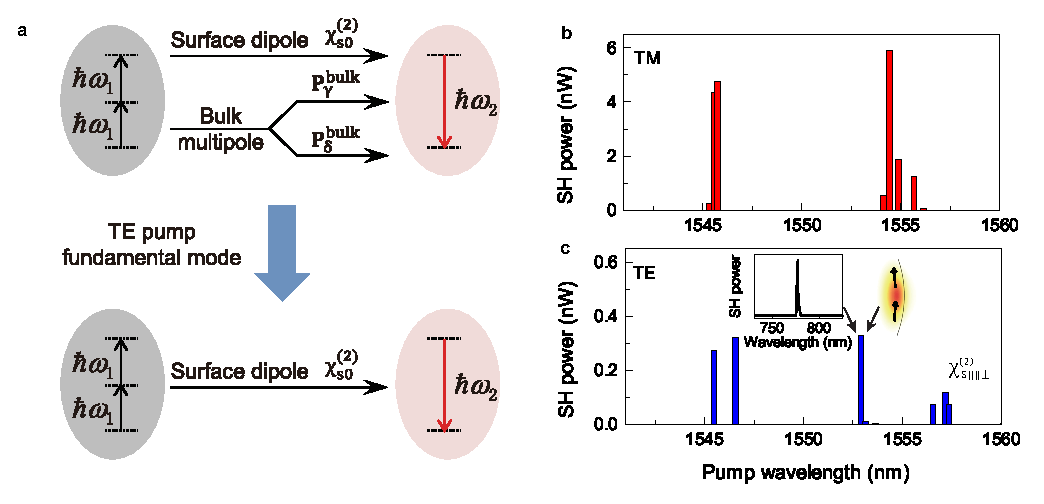
\includegraphics[width=16cm]{Fig3new.eps}
\caption{\textbf{Identification of surface nonlinearity from the bulk multipole response. a, }Origin of second-order nonlinearity and the method to obtain surface-only nonlinear coupling. \textbf{b,c,} Measured second harmonic power at the corresponding pump wavelength with TM (\textbf{b}) and TE (\textbf{c}) pump polarization respectively. Inset in \textbf{c}: Measured second harmonic spectrum (left), and field distribution of the target mode from numerical simulation(middle) and measurement (right).}
\label{pic:Fig3}
\end{figure*}


In order to distinguish the contributions of surface and bulk nonlinearity, we investigate the polarization dependence in SHG.  
In equation (\ref{eq:P2P1}), the nonlinear coupling strength from surface dipole response can be written as (see Supplementary Information)
\begin{equation}
g_{s0} = 2\frac{\omega_1^2}{\omega_2n^2}\frac{\int_{\mathrm{surface} } \mathbf{E}_{02}^*:\upchi^{(2)}_{s0}:\mathbf{E}_{01}\mathbf{E}_{01} \mathrm{d}	\mathbf{S}}{\int |\mathbf{E}_{02}|^2 \mathrm{d}	\mathbf{V}}
\end{equation}
where $\upchi^{(2)}_{s0}$ represents the surface nonlinear susceptibility, $\mathbf{E}_{0j}(\mathbf{x})$ denotes the  normalized electric field, and $n$ is the refractive index of the cavity material. 
The bulk multipole nonlinear polarization in silica can be expressed as $\mathbf{P}^{\mathrm{bulk}} =  \gamma\nabla(\mathbf{E}\cdot\mathbf{E})+\delta(\mathbf{E}\cdot\nabla)\mathbf{E}$ \cite{bloembergen1968optical}, where $\gamma$ and $\delta$ are the nonlinear coefficients. The first term $\mathbf{P}^{\mathrm{bulk}}_\gamma$ represents a longitudinal wave which can excite SH only at the surface. Therefore $\mathbf{P}^{\mathrm{bulk}}_\gamma$ can contribute to an effective surface susceptibility\cite{heinz1991second} $\upchi^{(2)}_s = \upchi^{(2)}_{s0}+\upchi^{(2)}_{s,\gamma}$, corresponding to an effective coupling strength of $g_s$. The coupling strength induced by the second term $\mathbf{P}^{\mathrm{bulk}}_\delta$ can be written as 
\begin{equation}
g_b =  2\frac{\omega_1^2}{\omega_2n^2}\frac{\delta \int \mathbf{E}_{02}^* \cdot (\mathbf{E}_{01}\cdot\nabla)\mathbf{E}_{01} \mathrm{d}	\mathbf{V}}{\int |\mathbf{E}_{02}|^2 \mathrm{d} \mathbf{V}}
\label{eq:gb}
\end{equation}
Thus the total second-order nonlinear coupling strength $g = g_s+g_b$, as shown in Fig. \ref{pic:Fig3}a.

The effective surface susceptibility tensor $\upchi^{(2)}_s$ contains three non-zero components $\upchi_{\perp \perp \perp}$, $\upchi_{\parallel \parallel \perp}$ and $\upchi_{\perp \parallel \parallel}$ \cite{heinz1991second}, where $\perp$ denotes the electric field direction perpendicular to the surface and $\parallel$ corresponds to the parallel direction. 
First, $\upchi_{\perp \parallel \parallel}$ can be ignored in studying SHG due to the non-degeneracy of transverse magnetic (TM) and  transverse electric (TE) pump modes.  
Second, $\upchi_{\perp \perp \perp}$ ($\upchi_{\parallel \parallel \perp}$) plays a major role when TM (TE) mode is pumped, which only generates the TM polarized second harmonic in both cases. 
TM modes are preferable in surface induced SHG because $\upchi_{\perp \perp \perp}$ is larger than $\upchi_{\parallel \parallel \perp}$ \cite{rodriguez2008calibration}. 
Considering the bulk nonlinear response induced by $\mathbf{P}^{\mathrm{bulk}}_\delta$, the coupling strength $g_b$ relies on the specific field distribution in the cavity and the generated SH exhibits the same polarization as the pump mode. 
Note that for TE polarization, the field direction is along the polar direction, so that the polar symmetry of modes prohibits the excitation of SH modes with an even polar distribution from $\mathbf{P}^{\mathrm{bulk}}_\delta$. 
While the TM pump modes, with electric field along the radial direction, can excite second harmonic without the above restriction.
Because of a stronger confinement in the radial direction than the polar direction and thus a larger divergence for most of the modes, TM modes tend to link with a larger $g_b$ than TE modes. 
Consequently, from both the surface and the bulk second-order nonlinearity, TM pump modes can generate stronger SH signals statistically. 
In the experiment, TM or TE modes from $1545$ nm to $1565$ nm are pumped separately by adjusting the polarization of the pump light.
The TM pump modes exhibit larger SH power, as shown in Fig. \ref{pic:Fig3}b and c, which agrees with the theoretical analysis.


The polarization dependence can be utilized to identify the surface nonlinearity from the bulk nonlinear response of both $\mathbf{P}^{\mathrm{bulk}}_\gamma$ and $\mathbf{P}^{\mathrm{bulk}}_\delta$. 
The former can be removed by selectively pumping a TE polarized mode since $\upchi^{(2)}_{s,\gamma}$ is absent in the susceptibility $\upchi_{\parallel \parallel \perp}$ \cite{heinz1991second}. 
The latter can also be discerned from the surface nonlinear response with a fundamental TE pump mode (angular number $l_1=m_1$), where SHG from $\mathbf{P}^{\mathrm{bulk}}_\delta$ is forbidden by the selection rule and the even polar field distribution of the SH mode (see Supplementary Information).  
In the measurement, a surface-only second harmonic is obtained deterministically by employ a fundamental TE pump mode at 1553.07 nm, as shown in the left inset in Fig. \ref{pic:Fig3}c.
Here the fundamental TE pump mode is confirmed experimentally by measuring the transmission while scanning the relative angular position of the pump fibre and the cavity, as illustrated in the right inset of Fig. \ref{pic:Fig3}c.
Additionally, $\mathbf{P}^{\mathrm{bulk}}_\delta$ can also be eliminated by measuring the polarization of the SH signal (see Supplementary Information). 

\begin{figure}[!ht]
\centering
%\captionsetup{singlelinecheck=no, justification = RaggedRight}
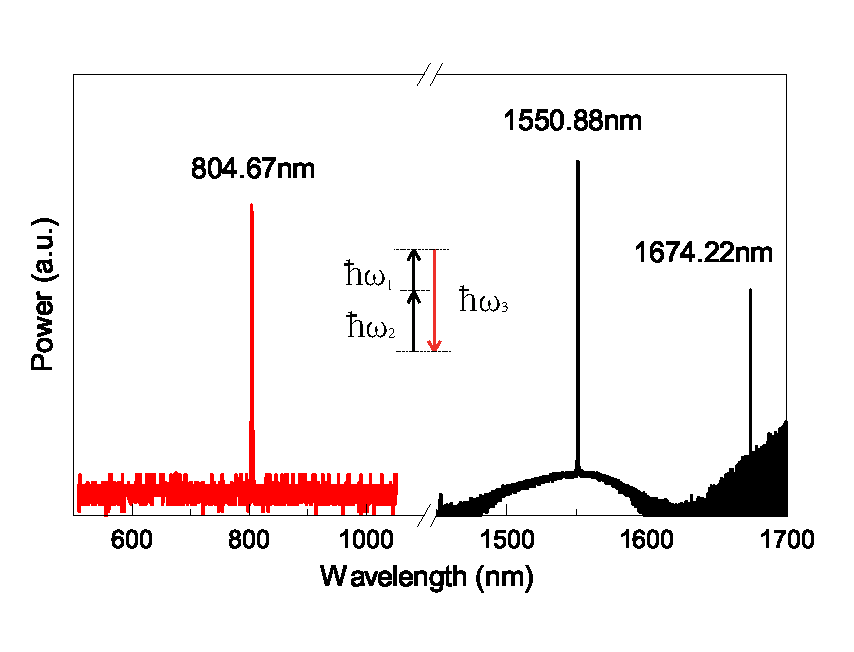
\includegraphics[width=8cm]{Fig4.eps}
\caption{\textbf{Measured spectra of second-order sum frequency generation (SFG). }The pump light ($\omega_1$) and Raman light ($\omega_R$) are summed to generate the SF signal ($\omega_2$) with an input power of $7.33$ mW.}
\label{pic:Fig4}
\end{figure}

With the second-order nonlinearity demonstrated above, sum frequency generation (SFG) also arises, assisted by a Raman signal. 
Shown in Fig. \ref{pic:Fig4} is a sum-frequency signal ($804.67$ nm), with the corresponding pump ($1550.88$ nm) and the stimulated Raman scattering ($1674.22$ nm).
The deviation of the sum-frequency wavelength from the expected value ($804.63$ nm) is much smaller than the resolution of the spectrometers.

For the first time, to the best of our knowledge, the second harmonic from the breaking of inversion symmetry at surface is deterministically observed in a silica microresonator without the influence of bulk multipoles. 
This work opens up a new direction to focus on the surface nonlinearity with double resonance enhancement, where the detectable SH signal under submilliwatt pump power enables to study surface properties and to detect molecules with unprecedented sensitivity. 
Moreover, the phase-matching method we used does not rely on the specific geometry and material of the cavity, making it a universal tool to develop surface nonlinear optics in various microcavity systems such as on-chip microtoroids, microdisks and microrings with different centrosymmetric materials like Si and Si$_3$N$_4$.
This work also shows great potential in studying CMOS-compatible quantum optics mediated by the second-order nonlinearity.
 
\bigskip
\noindent \textbf{\large Methods}

\noindent \textbf{Cavity fabrication and dual-fibre coupling system.}

\noindent The microsphere was fabricated directly on the tip of a standard single-mode telecom fibre. 
We melt the fibre with the CO$_2$ laser, and obtain the microsphere by melting the end of the fibre.
The dual fibres were fabricated respectively with standard single-mode fibre at the 1550 nm and 780 nm band, using different fabrication parameters.
%The signal fibre is fabricated together with the pump fibre but at a different relative position to the hydrogen flame. 
%In the process of fabricating the fibres, we monitored the transmission of both the fibres to achieve the single-mode condition at both the pump and SH wavelengths simultaneously.
The influence of the signal fibre to $Q$ is minor in the experiment.
For example, the intrinsic $Q$ of the pump mode in Fig. \ref{pic:Fig1}c before and after the incorporation of the signal fibre is $4.8\times10^7$ and $3.6\times10^7$.
The coupling between the signal fibre and the microsphere is adjusted while monitoring the transmission from the signal fibre with a tunable laser at the $780$ nm band.
The EMCCD and the pump laser are placed at the same side of the microsphere considering the linear momentum conservation requirement in SHG.

\noindent \textbf{Theoretical model and fitting.}

\noindent The SHG in the microresonator can be described by the following coupled mode equations
\begin{gather}
\frac{d{\alpha}_1}{dt} = [i(\omega_p-\omega_1)-\frac{\kappa_{10}+\kappa_{1e}}{2}]{\alpha}_1+\sqrt{\kappa_{1e}}s+ig^*{\alpha}_1{\alpha}_2^* \\
\frac{d{\alpha}_2}{dt} = [i(2\omega_p-\omega_2)-\frac{\kappa_{20}+\kappa_{2e}}{2}]{\alpha}_2-ig{\alpha}_1^2
\label{eq:cpmoder}
\end{gather}
where ${\alpha}_1$ denotes the field amplitude in the cavity, $s$ is the amplitude of the pump, and $\kappa_{j0}$ ($j = 1,2$) represents the intrinsic loss rate, which is related to the intrinsic $Q$ as $\kappa_{j0} = \omega_{j}/Q_{j0}$. 
To introduce the influence of thermal and Kerr effects, $\omega_1 =\omega_{10} -B_{11}|\alpha_1|^2$ and $\omega_2 =\omega_{20} -B_{12}|\alpha_1|^2$ are used to describe the red shift of the cavity modes.
$B_{11}$ and $B_{12}$ is determined by the effective thermal-induced refractive index change (${\partial n}/{\partial T})_{\mathrm{eff}}$ and the Kerr susceptibility $\chi_{\mathrm{Kerr}}$ (see Supplementary Information).
Equation (\ref{eq:cpmoder}) with the shifted $\omega_j$ is used to fit the measured data in Fig. \ref{pic:Fig2}c and d.
Fig. \ref{pic:Fig2}c deals with a small wavelength range so that the frequency shift of the SH mode is assumed to be proportion with the change of pump frequency $\Delta \omega_2 = D_{12}\Delta \omega_p$.
The theoretical curve is fitted under the condition of $Q_2\times(2-D_{12})=8.57\times 10^5$.
The critical input power in Fig. \ref{pic:Fig2}d is fitted to be $832.5$ $\upmu$W and the corresponding SH power is $381$ pW.

\bibliography{ref}

\bigskip
\noindent \textbf{\large Acknowledgment}

\noindent The authors thank Prof. T. F. Heinz, Prof. M. Lon$\mathrm{\check{c}}$ar, X. Yi for helpful discussion. 
This project was supported by the Ministry of Science
and Technology of China (Grants No. 2016YFA0301302,
No. 2013CB921904, and No. 2013CB328704) and the NSFC
(Grants No. 61435001, No. 11654003, and No. 11474011).

\bigskip
\noindent \textbf{\large Author contributions}

\noindent X. Z. performed the experiment and built the theoretical model. Y.-F. X. designed the
experiment and supervised the project. All authors contributed
to the discussion, analyzed the data, and wrote the
manuscript.
\end{document}

